\documentclass[11pt]{article}
\usepackage[letterpaper,margin=1in]{geometry}
\usepackage{amsmath,amssymb,bm,graphicx,booktabs,longtable,array}
\usepackage[hidelinks]{hyperref}
\newcommand{\ii}{\mathrm{i}}
\newcommand{\Dmat}{\bm{\Delta}}
\newcommand{\Tr}{\operatorname{tr}}
\usepackage{xcolor}
\newif\ifmarked
\IfFileExists{marked.flag}{\markedtrue}{\markedfalse}
\newcommand{\rev}[1]{\ifmarked{\color{blue}#1}\else#1\fi}
\newenvironment{revised}{\ifmarked\color{blue}\fi}{}
\renewcommand{\thetable}{S\arabic{table}}
\renewcommand{\thefigure}{S\arabic{figure}}
\title{Supplementary Material for\\``Phase-tuned delayed feedback for simultaneous linewidth and relative intensity noise suppression in semiconductor lasers''}
\author{Mauricio Herrera-Mar\'in}
\date{}
\begin{document}
\maketitle

\section*{S1. External-cavity mode and linearized matrices}

For $E(t)=Ae^{\ii\Omega t}$ and $N=N_s$, define $\theta=\phi+\Omega\tau$. The ECM equations are
\begin{align}
\theta-\phi+\kappa\tau(\alpha\cos\theta+\sin\theta)&=0,\\
N_s&=-\kappa\cos\theta,\\
A^2&=\frac{P-N_s}{1+2N_s},\\
\Omega&=-\kappa(\alpha\cos\theta+\sin\theta).
\end{align}
Let $c_r=\kappa\cos\theta$ and $c_i=-\kappa\sin\theta$. In the rotating frame, the matrices in
$\dot x=A_0x+A_1x(t-\tau)+B\eta$ are
\begin{equation}
A_0=\begin{pmatrix}
-c_r & c_i & A\\
-c_i & -c_r & \alpha A\\
-2\epsilon(1+2N_s)A & 0 & -\epsilon(1+2A^2)
\end{pmatrix},
\qquad
A_1=\begin{pmatrix}
c_r & -c_i & 0\\
c_i & c_r & 0\\
0&0&0
\end{pmatrix}.
\end{equation}
The characteristic matrix is $\Dmat(\lambda)=\lambda I-A_0-A_1e^{-\lambda\tau}$.

\begin{revised}\paragraph{ECM enumeration.} Equation (1) is solved for $\phi$ rather than for $\theta$: $\phi(\theta)=\theta+\kappa\tau(\alpha\cos\theta+\sin\theta)$. Every $\theta$ on one period defines exactly one ECM or antimode, so sampling $\theta$ enumerates all of them without root finding. Since $d\phi/d\theta=F=1+\kappa\tau(\cos\theta-\alpha\sin\theta)$ and $\min_\theta F=1-\kappa\tau\sqrt{1+\alpha^2}$, the map is monotone and the solution unique for every $\phi$ iff $C=\kappa\tau\sqrt{1+\alpha^2}<1$. Solutions with $F<0$ are antimodes. The principal ECM at $(\kappa,\phi)$ is defined by Newton continuation in $\kappa\tau$ at fixed $\phi$ from $\theta=\phi$; the continuation is declared terminated if $F$ reaches zero (saddle-node).\end{revised}

\section*{S2. Weak-feedback sensitivity}

At $\kappa=0$, $A=\sqrt P$, $N_s=0$, and the first derivative of the ECM intensity is
\begin{equation}
\left.\frac{dA^2}{d\kappa}\right|_{0}=(1+2P)\cos\phi.
\end{equation}
Differentiation of the exact phase-diffusion ratio gives
\begin{equation}
g_\varphi(\phi)=-\frac{1+2P}{P}\cos\phi-2\tau(\cos\phi-\alpha\sin\phi).
\end{equation}
For RIN, write $H_0(\ii\omega)=(\ii\omega I-A_0^{(0)})^{-1}B$. With
\begin{equation}
K_\phi(\omega)=A_{0,\kappa}+e^{-\ii\omega\tau}A_{1,\kappa},
\end{equation}
we use
\begin{equation}
\partial_\kappa H_0=H_0K_\phi H_0.
\end{equation}
The output row $C_{\rm RIN}=(2/A,0,0)$ is also differentiated. If $G_0=C_0H_0$ and
$G_\kappa=C_\kappa H_0+C_0\partial_\kappa H_0$, then
\begin{equation}
g_{\rm RIN}(\phi)=
\frac{2\,\mathrm{Re}\int_0^\infty \Tr[G_\kappa(\omega)G_0(\omega)^*]d\omega}
{\int_0^\infty \Tr[G_0(\omega)G_0(\omega)^*]d\omega}.
\end{equation}
For the baseline parameters, numerical quadrature gives
\begin{align}
g_\varphi&=-43.000000\cos\phi+160.000000\sin\phi,\\
g_{\rm RIN}&=-106.862441\cos\phi-344.419746\sin\phi.
\end{align}
The maximum residual from a first-harmonic fit is $2.8\times10^{-12}$. \rev{Writing $g_\varphi=a_\varphi\cos\phi+b_\varphi\sin\phi$ and $g_{\rm RIN}=a_R\cos\phi+b_R\sin\phi$ with $a_\varphi,a_R<0$, $b_\varphi>0$, $b_R<0$, the first-order simultaneous-suppression interval is
\begin{equation}
-\arctan\frac{a_R}{b_R}<\phi<\arctan\frac{-a_\varphi}{b_\varphi},
\end{equation}
i.e., $-0.09576\pi<\phi<0.08357\pi$ for the baseline. The values $-0.0944\pi$ and $0.0833\pi$ given in the original submission were the nearest points of a 721-point phase grid. Table~\ref{tab:fo} lists the first-order coefficients and intervals for the delays used in this work; for $\tau\gg1$ the upper bound tends to $\arctan(1/\alpha)=0.0780\pi$.} Table~\ref{tab:fdaudit} audits the formulas against finite differences at $\kappa=10^{-5}$.

\begin{table}[h]
\centering
\caption{First-order sensitivity audit.}\label{tab:fdaudit}
\begin{tabular}{ccccc}
\toprule
$\phi$ & $g_\varphi$ formula & finite difference & $g_{\rm RIN}$ formula & finite difference\\
\midrule
$-0.25$ & $-81.248$ & $-81.304$ & $-18.330$ & $-18.083$\\
$0$ & $-43.000$ & $-43.115$ & $-106.862$ & $-106.472$\\
$0.20$ & $-10.356$ & $-10.491$ & $-173.158$ & $-172.577$\\
$0.50$ & $38.972$ & $38.855$ & $-258.904$ & $-257.981$\\
\bottomrule
\end{tabular}
\end{table}

\begin{table}[h]
\centering
\caption{\rev{First-order coefficients and simultaneous-suppression intervals for several delays ($\alpha=4$, $\epsilon=0.005$, $P=1$).}}
\label{tab:fo}
\begin{revised}
\begin{tabular}{rrrrrcc}
\toprule
$\tau$ & $a_\varphi$ & $b_\varphi$ & $a_R$ & $b_R$ & lower bound$/\pi$ & upper bound$/\pi$\\
\midrule
10 & $-23$ & $80$ & $-49.603$ & $-116.042$ & $-0.1286$ & $0.0891$\\
20 & $-43$ & $160$ & $-106.862$ & $-344.420$ & $-0.0958$ & $0.0836$\\
40 & $-83$ & $320$ & $-96.128$ & $-408.912$ & $-0.0735$ & $0.0808$\\
200 & $-403$ & $1600$ & $-67.746$ & $-235.109$ & $-0.0893$ & $0.0785$\\
1000 & $-2003$ & $8000$ & $-71.606$ & $-266.454$ & $-0.0836$ & $0.0781$\\
\bottomrule
\end{tabular}
\end{revised}
\end{table}

\section*{S3. Phase diffusion and residue normalization}

For a simple characteristic root $\lambda_j$, the resolvent has the local expansion
\begin{equation}
\Dmat(s)^{-1}=\frac{v_ju_j^*}{u_j^*\Dmat'(\lambda_j)v_j}\frac{1}{s-\lambda_j}+O(1).
\end{equation}
At the neutral root, projection of white input noise gives
\begin{equation}
D_\varphi=\frac12\frac{u_0^*Qu_0}{|u_0^*\Dmat'(0)v_0|^2}.
\end{equation}
At a nonzero conjugate pair $\lambda_\pm$, integration of the retained transfer function gives
\begin{equation}
V_y^{(\pm)}=-\sum_{j,k\in\{+,-\}}
\frac{\Tr(CR_jBB^*R_k^*C^*)}{\lambda_j+\lambda_k^*}.
\end{equation}
The off-diagonal terms are retained. The pair reproduces $98.78\%$ of the trade-off RIN in the relaxation band and $94.49\%$ of the simultaneous-suppression RIN.

\begin{revised}
\paragraph{Factorization.}
With $\|u_j\|=\|v_j\|=1$, the delay-residue representation is
\begin{equation}
R_jB=\frac{v_j(B^*u_j)^*}{d_j},\qquad
V_{y,\mathrm{diag}}^{(\pm)}=
\sum_{j\in\{+,-\}}\frac{\|Cv_j\|^2\|B^*u_j\|^2}
{2|d_j|^2|\operatorname{Re}\lambda_j|}.
\end{equation}
Its ratio to the solitary value factorizes into a damping factor
$\operatorname{Re}\lambda^{(0)}/\operatorname{Re}\lambda$,
a delay-normalization factor $|d^{(0)}/d|^2$, and a source--output projection factor,
\begin{equation}
\frac{\|Cv\|^2\|B^*u\|^2}
{\|Cv^{(0)}\|^2\|B^*u^{(0)}\|^2}.
\end{equation}
The remaining cross-term factor compares the full conjugate-pair contribution with its
diagonal part, relative to the solitary laser. Table~\ref{tab:mech} reports the factors.

\begin{table}[h]
\centering
\caption{Factorization of the relaxation-pair RIN ratio.}
\label{tab:mech}
\small
\setlength{\tabcolsep}{3.5pt}
\begin{tabular}{lccccccc}
\toprule
State & damping & normalization & projection & cross & product & RIN (full) & $F^{-2}$\\
\midrule
Trade-off & 1.902 & 0.773 & 1.057 & 0.986 & 1.533 & 1.565 & 0.481\\
Joint suppression & 0.486 & 1.131 & 0.830 & 0.974 & 0.444 & 0.480 & 0.771\\
\bottomrule
\end{tabular}
\end{table}
The product equals the pair-only ratio; the difference to the full ratio is the non-pair contribution. Along the phase sweep at $\kappa\tau=0.18$ (main-text Fig.~4(d)), the damping factor crosses unity at $\phi=0.104\pi$ and the full RIN ratio at $\phi=0.080\pi$.\end{revised}

\section*{S4. Characteristic-root audit}

Roots were first seeded with an upwind transport-chain representation of the delay and then refined directly as zeros of $\det\Dmat(\lambda)$. The argument principle was evaluated on the rectangle
\begin{equation}
-0.05<\mathrm{Re}\,\lambda<0.02,\qquad |\mathrm{Im}\,\lambda|<0.5.
\end{equation}
For the solitary, trade-off, and simultaneous-suppression states, the winding number is three, corresponding to the neutral root and one conjugate relaxation pair. The minimum determinant magnitude on the contour is respectively $2.14\times10^{-4}$, $2.92\times10^{-4}$, and $2.44\times10^{-4}$. Table~\ref{tab:chain} shows convergence of the leading transport-chain root.

\begin{revised}\paragraph{Mikhailov count.} For the revision scans, stability is decided independently of the transport chain. Let $g(\lambda)=\det\Dmat(\lambda)/\lambda$, which is entire and removes the neutral root. Since the system is of retarded type, $g(\lambda)\sim\lambda^2$ for $|\lambda|\to\infty$ with $\mathrm{Re}\,\lambda>-\mu$, and the number of zeros with $\mathrm{Re}\,\lambda>-\mu$ is
\begin{equation}
N(\mu)=1-\frac{1}{2\pi}\Delta_{\omega=-W}^{W}\arg g(-\mu+\ii\omega),
\end{equation}
with $W=6$. The argument is unwrapped on a grid with at least $40W\tau/\pi+2000$ points, refined until successive phase increments are below $0.4$ rad. The stability margin is the largest $\mu$ with $N(\mu)=0$, found by bisection to $2\times10^{-5}$, capped at $\min(0.06,5/\tau)$. For the trade-off and simultaneous-suppression states this gives $0.003948$ and $0.015432$, compared with the refined roots $0.003944$ and $0.015428$.\end{revised}

\begin{table}[h]
\centering
\caption{Transport-chain convergence. Values are the root in the lower half-plane.}\label{tab:chain}
\begin{tabular}{cccc}
\toprule
State & chain cells & $\mathrm{Re}\,\lambda$ & $\mathrm{Im}\,\lambda$\\
\midrule
Trade-off & 30 & $-0.003908$ & $-0.104139$\\
& 60 & $-0.003923$ & $-0.104237$\\
& 120 & $-0.003932$ & $-0.104286$\\
Direct refinement & -- & $-0.003944$ & $-0.104336$\\
\midrule
Simultaneous suppression & 30 & $-0.015469$ & $-0.093979$\\
& 60 & $-0.015455$ & $-0.093765$\\
& 120 & $-0.015443$ & $-0.093658$\\
Direct refinement & -- & $-0.015428$ & $-0.093550$\\
\bottomrule
\end{tabular}
\end{table}

\section*{S5. Nonlinear stochastic delay simulations}

The full nonlinear equations were integrated in the ECM rotating frame using Euler--Maruyama. The delay was stored in a circular buffer with $\Delta t=0.02$, the record spacing was $0.1$, and 64 independent realizations were simulated for $T=3000$ after a burn-in of 400. The complex field noise amplitude was $\sigma=5\times10^{-4}$ in each quadrature. RIN and carrier variance were estimated after burn-in. Phase diffusion was estimated from time- and ensemble-averaged unwrapped-phase increments over lags from 150 to 780 normalized time units. Uncertainty bars in the main text are two standard errors across realizations. Table~\ref{tab:sde} compares the simulated and linear-resolvent ratios.

\begin{table}[h]
\centering
\caption{Direct nonlinear simulation and linear-resolvent ratios.}\label{tab:sde}
\begin{tabular}{lcccccc}
\toprule
& \multicolumn{2}{c}{linewidth} & \multicolumn{2}{c}{RIN} & \multicolumn{2}{c}{carrier}\\
State & simulation & linear & simulation & linear & simulation & linear\\
\midrule
Trade-off & 0.509 & 0.471 & 1.444 & 1.565 & 1.323 & 1.438\\
Simultaneous suppression & 0.824 & 0.750 & 0.478 & 0.480 & 0.514 & 0.518\\
\bottomrule
\end{tabular}
\end{table}

The stationary RIN and carrier results are insensitive to halving the time step within sampling uncertainty. The phase estimate is the slowest-converging quantity because it depends on long increments and contains bounded relaxation-mode contamination at finite lag.

\section*{S6. Noise-source, bandwidth, and fixed-output tests}

The field-noise matrix is
\begin{equation}
B_E=\begin{pmatrix}1&0\\0&1\\0&0\end{pmatrix}.
\end{equation}
A carrier-current source is represented by $B_N=(0,0,1)^T$. For the balanced mixed model, its scale is chosen so that field and carrier sources make equal contributions to the solitary integrated RIN; this gives a carrier-column scale of $\sqrt{0.0102245}$. Table~\ref{tab:noise} reports RIN ratios.

\begin{table}[h]
\centering
\caption{Integrated RIN ratios for alternative source models.}\label{tab:noise}
\begin{tabular}{lcc}
\toprule
Source model & Trade-off & Simultaneous suppression\\
\midrule
Field Langevin source & 1.565 & 0.480\\
Balanced field + carrier source & 1.744 & 0.490\\
\bottomrule
\end{tabular}
\end{table}

For normalized upper detection bandwidths $0.15$, $0.25$, $0.5$, $3$, and $200$, the trade-off ratios are $1.622$, $1.590$, $1.576$, $1.566$, and $1.565$, whereas the simultaneous-suppression ratios are $0.428$, $0.458$, $0.470$, $0.478$, and $0.480$.

At fixed output power $A=1$, the pump is adjusted to $P=1+3N_s$. The results are shown in Fig.~\ref{fig:fixed}.
\begin{figure}[h]
\centering
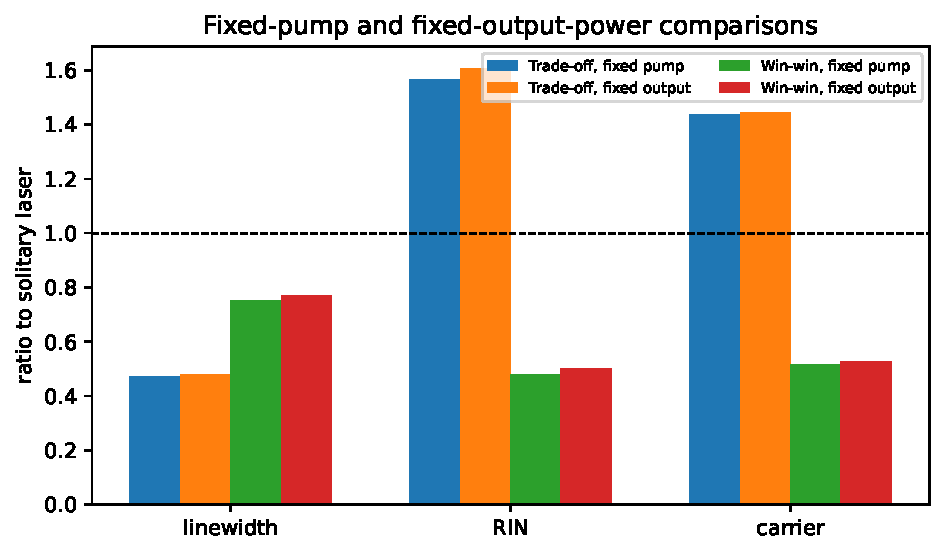
\includegraphics[width=0.78\textwidth]{figures/figS_fixed_output.pdf}
\caption{Comparison at fixed pump and fixed output power. The linewidth--RIN classification is unchanged.}\label{fig:fixed}
\end{figure}

\section*{S7. Extended robustness}

A coarse scan used $0<\kappa\leq0.009$ and 37 phases over $[-\pi,\pi]$. Gain compression was introduced through $G=N/(1+\eta |E|^2)$ in the field equation and the corresponding saturated stimulated-emission term in the carrier equation. Table~\ref{tab:robust} lists the best stable simultaneous-suppression point for each configuration.

\begin{longtable}{lcccc}
\caption{Extended robustness scan.}\label{tab:robust}\\
\toprule
Configuration & linewidth ratio & RIN ratio & stability margin & stable win--win fraction\\
\midrule
\endfirsthead
\toprule
Configuration & linewidth ratio & RIN ratio & stability margin & stable win--win fraction\\
\midrule
\endhead
$P=0.7$ & 0.681 & 0.507 & 0.0105 & 0.162\\
$P=1.0$ & 0.684 & 0.524 & 0.0137 & 0.153\\
$P=1.5$ & 0.686 & 0.567 & 0.0185 & 0.141\\
$\epsilon=0.003$ & 0.684 & 0.467 & 0.00834 & 0.160\\
$\epsilon=0.008$ & 0.684 & 0.606 & 0.0211 & 0.135\\
$\eta=0.05$ & 0.681 & 0.550 & 0.0128 & 0.144\\
$\eta=0.10$ & 0.679 & 0.579 & 0.0118 & 0.142\\
\bottomrule
\end{longtable}

\begin{revised}\paragraph{Linewidth-enhancement factor and delay; ECM audit.} The original statement for $\alpha\in\{2,4,6\}$ and $\tau\in\{10,20,40\}$ has been replaced by a scan that enumerates all ECMs and antimodes. For each combination, $\kappa\in\{0.001,\dots,0.009\}$ and 240 values of $\theta$ are sampled; each state is classified by the Mikhailov count of Sec.~S4. For every stable simultaneous-suppression state we record (i) whether $C<1$, (ii) whether it lies on the principal branch, (iii) the number of ECM solutions at its feedback phase, and (iv) whether another stable ECM coexists at that phase. Table~\ref{tab:audit} summarizes the results. Stable simultaneous-suppression states exist with $C<1$ in all nine combinations. Multi-ECM states occur only for $(\alpha,\tau)=(4,40)$ and $(6,40)$; there, five states each coexist with another stable ECM, and for $(6,40)$ 28 states belong to non-principal branches. The best state listed for each combination is restricted to $C<1$. The selected phase shifts with $\alpha$ and $\tau$, as expected from the ECM phase map.

\begin{table}[h]
\centering
\small
\caption{ECM audit of the $\alpha$--$\tau$ scan. $C_{\max}=0.009\tau\sqrt{1+\alpha^2}$. Columns 4--8 count stable simultaneous-suppression grid states: total, with $C<1$, on the principal branch, with more than one ECM at the same $\phi$, and coexisting with another stable ECM. The last four columns give the best state with $C<1$, by $(1-\text{linewidth ratio})+(1-\text{RIN ratio})$.}
\label{tab:audit}
\setlength{\tabcolsep}{4pt}
\begin{tabular}{rrcrrrrrcccc}
\toprule
$\alpha$ & $\tau$ & $C_{\max}$ & total & $C<1$ & principal & multi-ECM & multistable & $\kappa$ & $\phi/\pi$ & linewidth & RIN\\
\midrule
2 & 10 & 0.20 & 435 & 435 & 435 & 0 & 0 & 0.009 & $0.021$ & 0.792 & 0.707\\
2 & 20 & 0.40 & 374 & 374 & 374 & 0 & 0 & 0.009 & $0.085$ & 0.667 & 0.539\\
2 & 40 & 0.80 & 313 & 313 & 313 & 0 & 0 & 0.009 & $0.218$ & 0.512 & 0.582\\
4 & 10 & 0.37 & 245 & 245 & 245 & 0 & 0 & 0.009 & $0.087$ & 0.779 & 0.719\\
4 & 20 & 0.74 & 208 & 208 & 208 & 0 & 0 & 0.009 & $0.209$ & 0.657 & 0.548\\
4 & 40 & 1.48 & 162 & 108 & 162 & 6 & 5 & 0.006 & $0.295$ & 0.614 & 0.680\\
6 & 10 & 0.55 & 171 & 171 & 171 & 0 & 0 & 0.009 & $0.153$ & 0.778 & 0.718\\
6 & 20 & 1.09 & 137 & 121 & 137 & 0 & 0 & 0.008 & $0.296$ & 0.695 & 0.568\\
6 & 40 & 2.19 & 108 & 48 & 80 & 41 & 5 & 0.004 & $0.306$ & 0.734 & 0.735\\
\bottomrule
\end{tabular}
\end{table}\end{revised}

\section*{S8. Device-scale illustration}

A photon lifetime $\tau_p=2.5$ ps is used only to demonstrate the dimensional conversion. Then $\epsilon=0.005$ corresponds to a carrier lifetime of $500$ ps, $\tau=20$ corresponds to an external round trip of $50$ ps, and normalized angular frequency maps to $f=\omega/(2\pi\tau_p)$. The white-noise strength is calibrated so that the solitary Lorentzian linewidth is $2$ MHz. The resulting values are listed in Table~\ref{tab:dim}:

\begin{table}[h]
\centering
\caption{Illustrative dimensional values.}\label{tab:dim}
\small\setlength{\tabcolsep}{4pt}
\begin{tabular}{lccc}
\toprule
State & linewidth (MHz) & RIN-peak frequency (GHz) & RIN peak (dBc/Hz)\\
\midrule
Solitary & 2.000 & 6.366 & $-130.76$\\
Trade-off & 0.941 & 6.641 & $-126.07$\\
Simultaneous suppression & 1.500 & 6.048 & $-137.20$\\
\bottomrule
\end{tabular}
\end{table}

These numbers are not a fit to a particular device. They show that the normalized ratios correspond to realistic semiconductor-laser time scales and to directly measurable linewidth and RIN quantities.

\begin{revised}
\section*{S9. Finite-feedback range of the criterion and tolerances}

For $\tau\in\{20,200,1000\}$ and $\kappa\tau\in[0.002,0.24]$, all ECMs are sampled in $\theta$ (361, 241, and 181 points, respectively). The stable simultaneous-suppression set is located on the grid, and its edges are refined by Brent's method on the linewidth or RIN ratio minus one. Table~\ref{tab:windows} lists the results for $\tau=20$; the complete tables are in the repository (\texttt{windows\_tau*.csv}). In all cases the edges are set by the noise criteria, not by stability.

\begin{table}[h]
\centering
\caption{Stable simultaneous-suppression window for $\tau=20$: full resolvent versus first-order prediction. ``Mapped'' gives the first-order $\theta$ bounds converted to $\phi$ through the ECM phase map.}
\label{tab:windows}
\begin{tabular}{ccccccc}
\toprule
$\kappa\tau$ & $\theta_-/\pi$ & $\theta_+/\pi$ & $\phi_-/\pi$ & $\phi_+/\pi$ & mapped $\phi_-/\pi$ & mapped $\phi_+/\pi$\\
\midrule
0.002 & $-0.0959$ & $0.0836$ & $-0.0937$ & $0.0862$ & $-0.0935$ & $0.0862$\\
0.020 & $-0.0976$ & $0.0836$ & $-0.0752$ & $0.1098$ & $-0.0733$ & $0.1098$\\
0.050 & $-0.1005$ & $0.0836$ & $-0.0449$ & $0.1492$ & $-0.0397$ & $0.1492$\\
0.100 & $-0.1057$ & $0.0836$ & $0.0043$ & $0.2148$ & $0.0164$ & $0.2148$\\
0.150 & $-0.1113$ & $0.0836$ & $0.0517$ & $0.2804$ & $0.0725$ & $0.2804$\\
0.180 & $-0.1149$ & $0.0836$ & $0.0792$ & $0.3198$ & $0.1061$ & $0.3198$\\
0.200 & $-0.1174$ & $0.0836$ & $0.0972$ & $0.3460$ & $0.1286$ & $0.3460$\\
0.240 & $-0.1226$ & $0.0836$ & $0.1320$ & $0.3985$ & $0.1735$ & $0.3985$\\
\bottomrule
\end{tabular}
\end{table}

\paragraph{Tolerances.} Along the principal ECM at $\kappa\tau=0.18$, the simultaneous-suppression interval is $0.0792\pi<\phi<0.3198\pi$. A phase error $\delta\phi$ corresponds to a round-trip path error $\lambda\,\delta\phi/(2\pi)$ and to a reflector displacement of half that value. Table~\ref{tab:tol} gives the conversion for common wavelengths. At fixed $\phi=0.25\pi$, Table~\ref{tab:kcont} follows the principal ECM in $\kappa\tau$; the ECM remains the only solution up to $\kappa\tau=0.40$.

\begin{table}[h]
\centering
\caption{Phase tolerance of the simultaneous-suppression state $(\kappa\tau,\phi)=(0.18,0.25\pi)$.}
\label{tab:tol}
\begin{tabular}{lccc}
\toprule
& $\lambda=850$ nm & $1310$ nm & $1550$ nm\\
\midrule
Reflector displacement, $\delta\phi=+0.070\pi$ (linewidth edge) & 14.8 nm & 22.8 nm & 27.0 nm\\
Reflector displacement, $\delta\phi=-0.171\pi$ (RIN edge) & 36.3 nm & 55.9 nm & 66.2 nm\\
\bottomrule
\end{tabular}
\end{table}

\begin{table}[h]
\centering
\caption{Continuation of the principal ECM in $\kappa\tau$ at fixed $\phi=0.25\pi$, $\tau=20$.}
\label{tab:kcont}
\begin{tabular}{ccccccc}
\toprule
$\kappa\tau$ & $\theta/\pi$ & $F$ & linewidth & RIN & carrier & margin\\
\midrule
0.04 & $0.2014$ & 0.938 & 1.132 & 0.644 & 0.685 & 0.0126\\
0.08 & $0.1475$ & 0.929 & 1.147 & 0.521 & 0.578 & 0.0161\\
0.12 & $0.0927$ & 0.977 & 1.029 & 0.477 & 0.535 & 0.0171\\
0.16 & $0.0414$ & 1.076 & 0.844 & 0.472 & 0.519 & 0.0163\\
0.18 & $0.0180$ & 1.139 & 0.750 & 0.480 & 0.518 & 0.0154\\
0.20 & $-0.0039$ & 1.210 & 0.663 & 0.494 & 0.521 & 0.0145\\
0.24 & $-0.0426$ & 1.366 & 0.517 & 0.538 & 0.541 & 0.0125\\
0.28 & $-0.0756$ & 1.536 & 0.407 & 0.605 & 0.579 & 0.0105\\
0.32 & $-0.1035$ & 1.712 & 0.326 & 0.703 & 0.640 & 0.0087\\
0.36 & $-0.1274$ & 1.893 & 0.265 & 0.843 & 0.732 & 0.0070\\
0.40 & $-0.1481$ & 2.075 & 0.220 & 1.052 & 0.871 & 0.0055\\
\bottomrule
\end{tabular}
\end{table}

\section*{S10. Long external cavities}

Delays $\tau=200$ and $1000$ correspond to about 3 and 16 solitary relaxation periods ($2\pi/\omega_R\approx63$). The resolvent quadrature uses a uniform grid with spacing $\min(2\times10^{-4},0.03/\tau)$ up to $\omega=0.6$, which resolves the external-cavity ripple of period $2\pi/\tau$, followed by a logarithmic grid to $\omega=200$. Stability is decided by the Mikhailov count of Sec.~S4, whose grid scales with $\tau$.

\paragraph{Fixed $\kappa\tau$.} For $\kappa\tau\le0.24$ the ECM is unique. The full-resolvent window in $\theta$ is $[-0.0893\pi,0.0785\pi]$ to $[-0.0898\pi,0.0785\pi]$ for $\tau=200$ and $[-0.0836\pi,0.0781\pi]$ for $\tau=1000$ over the whole range, compared with the first-order bounds $[-0.0893\pi,0.0785\pi]$ and $[-0.0836\pi,0.0781\pi]$ (Table~\ref{tab:fo}). For $\kappa\tau=0.18$ and $\theta=0.018\pi$, the linewidth, RIN, and carrier ratios are $0.769$, $0.933$, $0.935$ ($\tau=200$) and $0.770$, $0.985$, $0.985$ ($\tau=1000$).

\paragraph{Fixed $\kappa$, multi-ECM regime.} For the settings in Table~\ref{tab:longS}, 1440 values of $\theta$ are sampled, antimodes are discarded, and every remaining ECM is classified by the Mikhailov count. Figure~\ref{fig:long} shows the linewidth and RIN ratios of all stable ECMs. The window edges in Table~\ref{tab:longS} are limited by the $\theta$ grid spacing, $0.0014\pi$.

\begin{table}[h]
\centering
\caption{Long-cavity scans with all ECMs enumerated. $N_s$ is the number of stable ECMs at the feedback phase of the in-phase mode $\theta=0$; linewidth and RIN ratios refer to that mode.}
\label{tab:longS}
\begin{tabular}{rccccccc}
\toprule
$\tau$ & $\kappa$ & $\kappa\tau$ & $C$ & $N_s$ & $\theta$ window$/\pi$ & linewidth & RIN\\
\midrule
200 & 0.001 & 0.2 & 0.82 & 1 & $[-0.089,\,0.078]$ & 0.692 & 0.938\\
200 & 0.002 & 0.4 & 1.65 & 2 & $[-0.089,\,0.078]$ & 0.507 & 0.884\\
200 & 0.005 & 1.0 & 4.12 & 1 & $[-0.090,\,0.078]$ & 0.246 & 0.761\\
200 & 0.009 & 1.8 & 7.42 & 1 & $[-0.092,\,0.078]$ & 0.124 & 0.650\\
1000 & 0.0005 & 0.5 & 2.06 & 2 & $[-0.083,\,0.078]$ & 0.444 & 0.966\\
1000 & 0.001 & 1.0 & 4.12 & 2 & $[-0.083,\,0.078]$ & 0.249 & 0.935\\
1000 & 0.002 & 2.0 & 8.25 & 3 & $[-0.083,\,0.078]$ & 0.110 & 0.880\\
\bottomrule
\end{tabular}
\end{table}

\begin{figure}[h]
\centering
\includegraphics[width=\textwidth]{figures/figS2_long_cavity.pdf}
\caption{Linewidth (dots) and RIN (crosses) ratios of stable ECMs versus total return phase for $\tau=200$, $\kappa=0.005$ (left) and $\tau=1000$, $\kappa=0.001$ (right), reconstructed with 1440 phase samples per setting. The shaded band marks the first-order simultaneous-suppression interval for the same delay; only modes with $F>0$ and zero non-neutral unstable characteristic roots are shown. Displayed ratios are limited to $2.2$ for readability.}
\label{fig:long}
\end{figure}

\paragraph{Nonlinear simulations.} The simulations of Sec.~S5 were repeated with the ECM specified by $\theta$, so that a selected mode is followed even when other ECMs coexist. The history was initialized on the selected ECM, $\Delta t=0.02$, $\sigma=5\times10^{-4}$, and 128 independent realizations were simulated per state. Burn-in and record length were 2000 and $10^{5}$ for $\tau=200$ and 10000 and $4\times10^{5}$ for $\tau=1000$. Phase diffusion was obtained from the slope of the phase mean-square displacement over lags from 3$\tau$ to 12$\tau$, after removing a small residual offset of the mean optical frequency that is common to all realizations and would otherwise add a term quadratic in the lag; changing this window to $2\tau$--$8\tau$ or $5\tau$--$20\tau$ changes the linewidth ratios by less than their two-standard-error uncertainty (file \texttt{lag\_sensitivity.csv}). Intensity and carrier variances were accumulated at every time step after burn-in. Table~\ref{tab:sdelong} compares the results with the linear resolvent; the solitary reference was simulated with the same settings.

\begin{table}[h]
\centering
\small
\caption{Nonlinear stochastic simulations in the long-cavity regime (ratios to the solitary laser; $\pm$ two standard errors).}
\label{tab:sdelong}
\setlength{\tabcolsep}{4pt}
\begin{tabular}{rclcccccc}
\toprule
$\tau$ & $\kappa$ & ECM & linewidth & lin. & RIN & lin. & carrier & lin.\\
\midrule
200 & 0.005 & trade-off, $\theta=-0.156\pi$ & $0.070\pm0.004$ & 0.070 & $1.371\pm0.013$ & 1.369 & $1.353\pm0.013$ & 1.352\\
200 & 0.005 & in-phase, $\theta=0$ & $0.238\pm0.014$ & 0.246 & $0.756\pm0.006$ & 0.761 & $0.760\pm0.007$ & 0.764\\
1000 & 0.001 & trade-off, $\theta=-0.156\pi$ & $0.066\pm0.004$ & 0.070 & $1.069\pm0.005$ & 1.069 & $1.068\pm0.005$ & 1.069\\
1000 & 0.001 & in-phase, $\theta=0$ & $0.248\pm0.017$ & 0.249 & $0.933\pm0.004$ & 0.935 & $0.933\pm0.004$ & 0.934\\
\bottomrule
\end{tabular}
\end{table}
\end{revised}

\section*{\rev{S11}. Reproducibility files}

The original public repository provides the ECM solver, delay-resolvent quadrature,
phase-diffusion calculation, root and stability audits, stochastic simulations,
noise-source tests, robustness analyses, numerical tables, and figure scripts.
The companion revision reproducibility archive adds the corresponding numerical
outputs and the following \rev{programs: \path{rev_core.py} (shared ECM and resolvent routines),
\path{rev_windows.py} (finite-feedback windows), \path{rev_firstorder.py} (weak-feedback sensitivity),
\path{rev_tolerance.py} (experimental tolerances), \path{rev_mechanism.py} (modal factorization),
\path{rev_ecm_audit.py} (ECM enumeration), \path{rev_longcavity_strong.py} (long cavities),
and \path{rev_sde.py} (stochastic validation).}

\end{document}
